\documentclass[12pt]{article}
\usepackage[left=2cm, right=2cm, top=2cm]{geometry}
\usepackage[utf8]{inputenc} 
\usepackage{graphicx} % to include images
\usepackage{amsmath} % For math mode
\usepackage{caption} % For captions
\usepackage{subcaption} % To use caption while using mini page
\usepackage{amssymb} % To use math symbols
\usepackage{multirow} %To combine multiple rows in a table
\usepackage[table]{xcolor} %To color rows / columns in table
\usepackage{titling} %To vertically center the title page
\usepackage{hyperref} %for URL


%----------------------------MATLAB TEMPLATE -------------------------------------
\usepackage{listings}
\usepackage{color} %red, green, blue, yellow, cyan, magenta, black, white
\definecolor{mygreen}{RGB}{28,172,0} % color values Red, Green, Blue
\definecolor{mylilas}{RGB}{170,55,241}
%-----------------------------------------------------------------------------------------

\title{ECE 8540 Analysis of Tracking Systems \\ 
	Assignment 3}
\author{Vivek Koodli Udupa \\ C12768888}
\date{September - 25, 2018 }

%To make the title page center vertically centered
\renewcommand\maketitlehooka{\null\mbox{}\vfill}
\renewcommand\maketitlehookd{\vfill\null}

\begin{document}

%Displaying Title
\begin{titlepage}
\maketitle
\pagenumbering{gobble}% Remove page numbers (and reset to 1)
\end{titlepage}
\pagenumbering{arabic}% Arabic page numbers (and reset to 1)

%Beginning of the report
\section{Introduction}
%what is the problem? - non linear model fit?
This report considers the problem of modeling a linear fit. Models are tools that are used to easily understand scientific ideas or to explain how data and events are related to each other. Scientists often use models to predict what might happen in a particular circumstance based on current available information. Weather prediction is a good example where a forecast is given based on past and current weather conditions. \\
\\
The mathematical models can be linear or non-linear in nature. A line of the form $y = ax + b$ and an exponential function of the form $y = e^{ax}$ are examples for linear and non-linear models respectively. The difference between linear and non-linear models is not straight forward as it seems. It would be wrong to assume that linear equations only produce straight lines whereas non linear equations produce curves. Linear equations can produce curved lines too! So in that case how do we know whether a model is linear or non-linear?\\
\\
Statistically speaking, a model is linear in terms of its parameters if all its terms are either constants or a parameter multiplied by an independent variable. $y = a_0 + a_1 x_1 + .... + a_n x_x$ represents a linear model. Model of any other form is non-linear[1]. \\
\\
Through the course of the report, we will try to fit a model to the given data set by formulating appropriate matrices and finding the model parameters using normal equations. Initially a 2D line is fit to the given data set of five points. Later the effect of an additional point on the slope of the line will be observed. For the final part of the lab, we will fit an equation of the form $y = ax^b$ by converting the equation into linear in terms of its parameters and then computing the parameters.
 
\section{Methods}
\begin{figure}[h]
\centering
	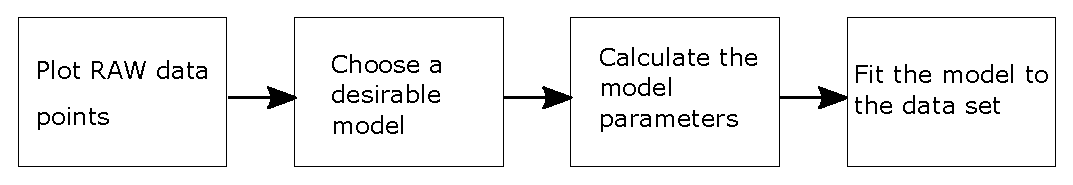
\includegraphics[width=\textwidth]{flowchart}
	\caption{Flowchart for model fitting }
	\label{fig:flowchart}
\end{figure}
\noindent
This section walks us through the entire process of fitting a model to the given data set. The process can be divided into 4 stages, as shown in Figure \ref{fig:flowchart}. Initially, the raw data is plotted for visualization. This gives us a basic idea of what the model must look like. Based on this visual analysis, a desirable model that most likely fits is chosen. Once we have the equation representing the model, we must calculate the values of the constants and other included parameters. This is the basic idea of how to fit a model. We will go through these steps in greater detail as we model the fit for particular data set. We were given two data sets for this lab. Data set 1 is used for part A and part B of the lab and data set 2 is used for the part C of the lab. 

\subsection{General solution to normal equations} \label{ss:general}
The equation of a line is a special case of a generalized fitting of any function consisting of linear combination of terms. 
\begin{equation}
 y = a_1 f_1 (x) + a_2 f_2 (x) + ...... + a_M f_M (x)
\label{eq:general}
\end{equation}
where $a_1 ... a_M$ are linear unknowns. The terms $f_1(x) .... f_M(x)$ are called basis functions. There is no need for the basis function to be linear. But the unknowns must all be linear constants. \\
\\
Given a set of data points, say $(x_i , y_i) \quad i = 1...N$, we wish to find the solution to Equation \ref{eq:general} that best fits the data.  \\
\\
Now we define the residual $e_i$ for each point as :
\begin{equation}
e_i = \left(y_i - \sum_{j = 1}^M a_j f_j (x_i)\right)
\end{equation}\\
To find the difference between the collective set of data and the best fitting solution, we define the chi-squared error metric:
\begin{equation}
\chi^2 (a_1, a_2, ....., a_M) = \sum_{i = 1}^N \left(y_i - \sum_{j = 1}^M a_j f_j (x_i)\right)^2
\end{equation}\\
The best possible values for the unknowns can be found by using differential equations to solve for the minimum chi-squared error. We take the partial derivatives of $\chi^2$ with respect to $a_1....a_M$, equate them to zero and solve for $a_1....a_M$. \\
In general form, the set of M equations can be written as :
\begin{equation}
\forall K = 1...M \quad  \frac{\partial \chi^2}{\partial a_k} = \sum_{i = 1}^N 2 \left(y_i - \sum_{j = 1}^M a_j f_j (x_i)\right) (-f_k(x_i))
\end{equation}\\
To solve for the unknowns, we set all the equations to zero: 
\begin{equation}
\forall K = 1...M \quad  \frac{\partial \chi^2}{\partial a_k} = \sum_{i = 1}^N (f_k(x_i))\left(y_i - \sum_{j = 1}^M a_j f_j (x_i)\right) = 0
\end{equation}\\
Rearranging the terms and expanding the sums, we obtain 
\begin{equation}
\forall K = 1...M \quad  \sum_{i=1}^N f_k(x_i)y_i = \sum{i = 1}^N \sum_{j = 1}^M f_k (x_i) f_j(x_i)a_j
\label{eq:normal}
\end{equation}\\
For the purpose of simplification, we will use matrix notation. We define the following matrices:
\begin{equation}
A = 
	\begin{bmatrix}
		f_1(x_1) & f_2(x_1) &....&f_M(x_1) \\ 
		f_1(x_2) & f_2(x_2) &....&f_M(x_2) \\
		. & .  & & . \\
		. & .  & & . \\
		. & .  & & . \\		
		f_1(x_N) & f_2(x_N) &....&f_M(x_N) \\	
	\end{bmatrix}
\label{eq:matA}
\end{equation}
\\
\begin{equation}
x = 
	\begin{bmatrix}
		a_1 \\
		a_2 \\
		. \\
		. \\
		. \\
		a_M
	\end{bmatrix}
\label{eq:matx}
\end{equation}
\\
\begin{equation}
b = 
	\begin{bmatrix}
		y_1 \\
		y_2 \\
		. \\
		. \\
		. \\
		y_M
	\end{bmatrix}
\label{eq:matb}
\end{equation}
Using the matrices, we can rewrite equation \ref{eq:normal} in matrix form as:
\begin{equation}
A^Tb = A^TAx
\label{eq:matrixform}
\end{equation}
Our goal is to solve for the unknowns in matrix x.  Note that $A^TA$ is by definition a square matrix and is therefore invertible. Multiplying both sides of equation \ref{eq:matrixform} by this inverse and then rearranging gives:
\begin{equation}
(A^T A)^{-1} A^T Ax = (A^T A)^{-1}A^Tb
\end{equation}
Any matrix multiplied by its inverse yields the identity matrix. Thus the left side of the equation simplifies to:
\begin{equation}
x = (A^T A)^{-1} A^T b
\label{eq:solution}
\end{equation}
Equation \ref{eq:solution} is known as the solution to the normal equations. Given properly constructed matrices A, x and b, the solution to any problem in the form of equation \ref{eq:general} can be found using equation \ref{eq:solution}.
\subsection{Part A and Part B}
%SEPERATE THE  PLOTS. MAKE IT TWO SEPARATE FIGURES AND REMOVE THE TITLE
\begin{figure}[h]
\centering
\begin{minipage}{0.5\textwidth}
\centering	
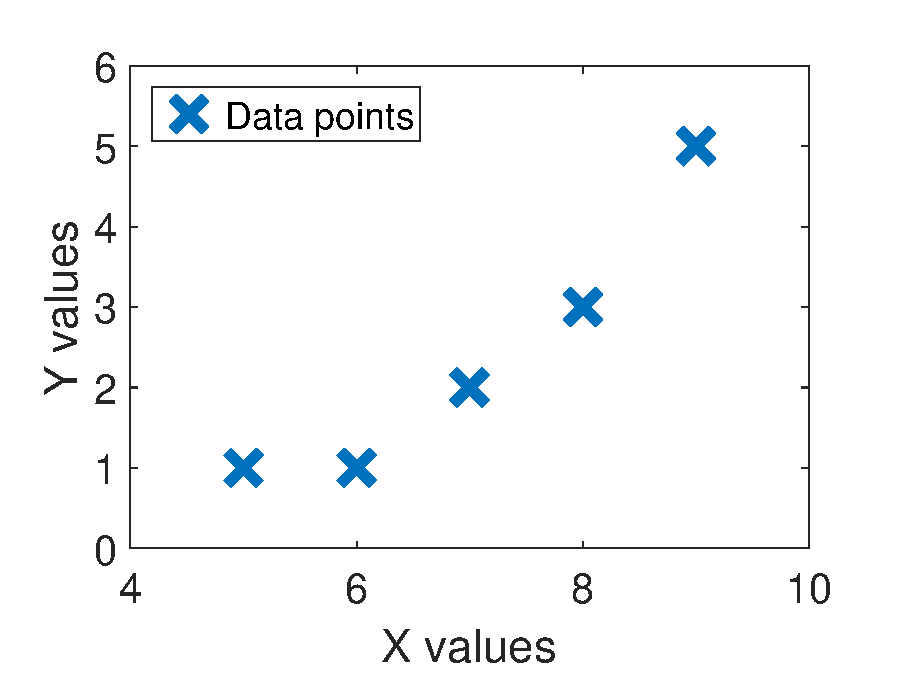
\includegraphics[scale=0.50]{dataA}
	\caption{Plot of Raw data set A points }
	\label{fig:dataA}
\end{minipage}%
%\begin{figure}[h]
\centering	
\begin{minipage}{0.5\textwidth}
\centering	
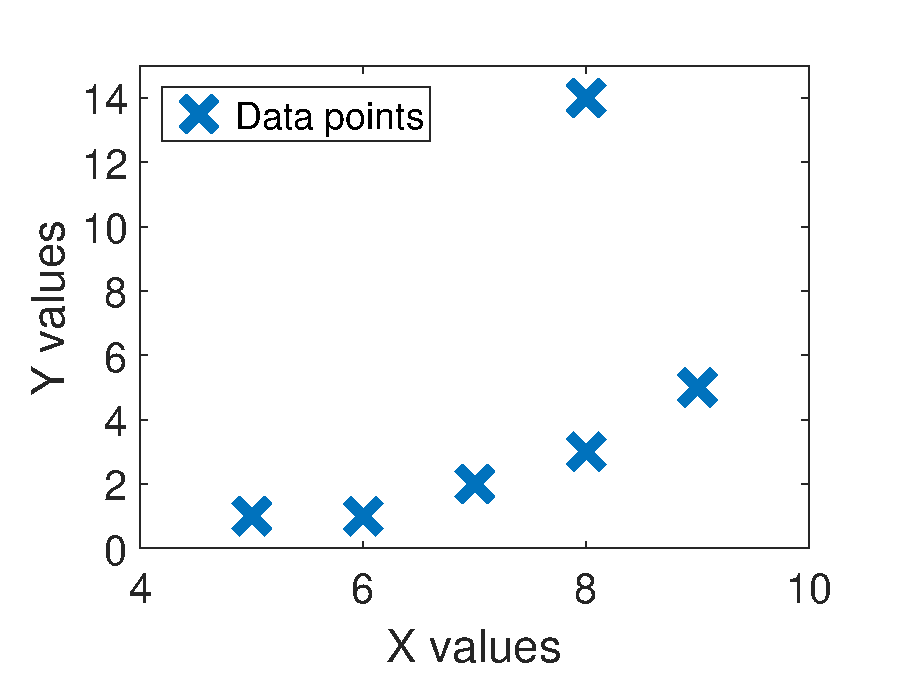
\includegraphics[scale=0.50]{dataB}
	\caption{Plot of Raw data set B points }
	\label{fig:dataB}
\end{minipage}
\end{figure}

Data set A points: (5 , 1); (6 , 1); (7 , 2); (8 , 3); (9 , 5) \\
Data set B points: (5 , 1); (6 , 1); (7 , 2); (8 , 3) ;(9 , 5); (8 , 14) \\
Figure \ref{fig:dataA} and Figure \ref{fig:dataB} represent the plot of Data set A and Data set B respectively.  \\
\\
The first step in modeling a fit was to visualize the data. The next step is to find a model that might fit this visualization. \\ \\
The y value of the data points seems to increase linearly as we traverse along the x-axis. Thus a 2D line of the form $y = ax + b$ might fit well. It is to be noted that the point (8,14) in Part B data set is considered as an outlier as its value is far off from other points. \\
\\
Now we will formulate the matrices that were specified in equation \ref{eq:matA}, equation \ref{eq:matx} and equation \ref{eq:matb} .
\begin{equation}
A  = 
	\begin{bmatrix}
	x_1 & 1 \\
	x_2 & 1 \\
	. & . \\
	. & . \\
	x_N & 1
	\end{bmatrix}
\end{equation} \\
\begin{equation}
x  = 
	\begin{bmatrix}
	a \\
	b
	\end{bmatrix}
\end{equation} \\
\begin{equation}
A  = 
	\begin{bmatrix}
	y_1 \\
	y_2 \\
	.  \\
	.  \\
	y_N
	\end{bmatrix}
\end{equation}
Now we shall fill in the matrices with appropriate values from data set A. 
\begin{equation}
A  = 
	\begin{bmatrix}
	5 & 1 \\
	6 & 1 \\
	7 & 1 \\
	8 & 1\\
	9 & 1
	\end{bmatrix}
\end{equation} \\
\begin{equation}
b  = 
	\begin{bmatrix}
	1 \\
	1 \\
	2 \\
	3 \\
	5
	\end{bmatrix}
\end{equation}\\
\begin{equation}
x_u  = 
	\begin{bmatrix}
	a \\
	b
	\end{bmatrix}
\end{equation} \\
With the above matrices, the value of $x_u$ can be calculated using equation \ref{eq:solution}. Using MATLAB for calculations, we get the following values for $x_u$ : 
\begin{equation}
x_u = 
	\begin{bmatrix}
	 1.00\\
	-4.60 \\
	\end{bmatrix}
\end{equation}
\noindent
Therefore the 2D line fit for Data set A is given by 
\begin{equation}
y_i = 1.00(x_i) - 4.60
\label{ans:A}
\end{equation} 
\noindent
Following the similar method, the matrices constructed for Part B take the following form:
\begin{equation}
A  = 
	\begin{bmatrix}
	5 & 1 \\
	6 & 1 \\
	7 & 1 \\
	8 & 1\\
	9 & 1\\
	8 & 14
	\end{bmatrix}
\end{equation} \\
\begin{equation}
b = 
	\begin{bmatrix}
	1 \\
	1 \\
	2 \\
	3 \\
	5 \\
	14
	\end{bmatrix}
\end{equation}\\
\begin{equation}
x_u  = 
	\begin{bmatrix}
	a \\
	b
	\end{bmatrix}
\end{equation} \\
\noindent
By using the same method used for Part A, we find the value of  the unknowns for Part B of the lab as follows: 
\begin{equation}
x_u  = 
	\begin{bmatrix}
	1.8154 \\
	-8.6769
	\end{bmatrix}
\end{equation} \\
\noindent
Thus the line fit for Part B of the lab takes the form :
\begin{equation}
y_i = 1.8154(x_i) - 8.6769
\label{ans:B}
\end{equation}

\subsection{Part C}
For the third part of the lab, the data set named \lq\lq{83people-all-meals.txt}\rq\rq{} is given. The data are for 3,398 meals eaten by 83 different people.  The first column is the participant ID, the second column is the meal ID.  The third column is the number of bites taken in the meal, and the fourth column is the number of kilo calories consumed.  \\ \\
In order to visualize the data, we have to plot the data. We will be plotting column 3 (i.e., number of bites taken in a meal) against the dividend of column 4 and column 3 (i.e., kilo-calories consumed per bite). This will give us the statistic of number of kilo-calories consumed per bite.  

\begin{figure}[b!]
\centering
	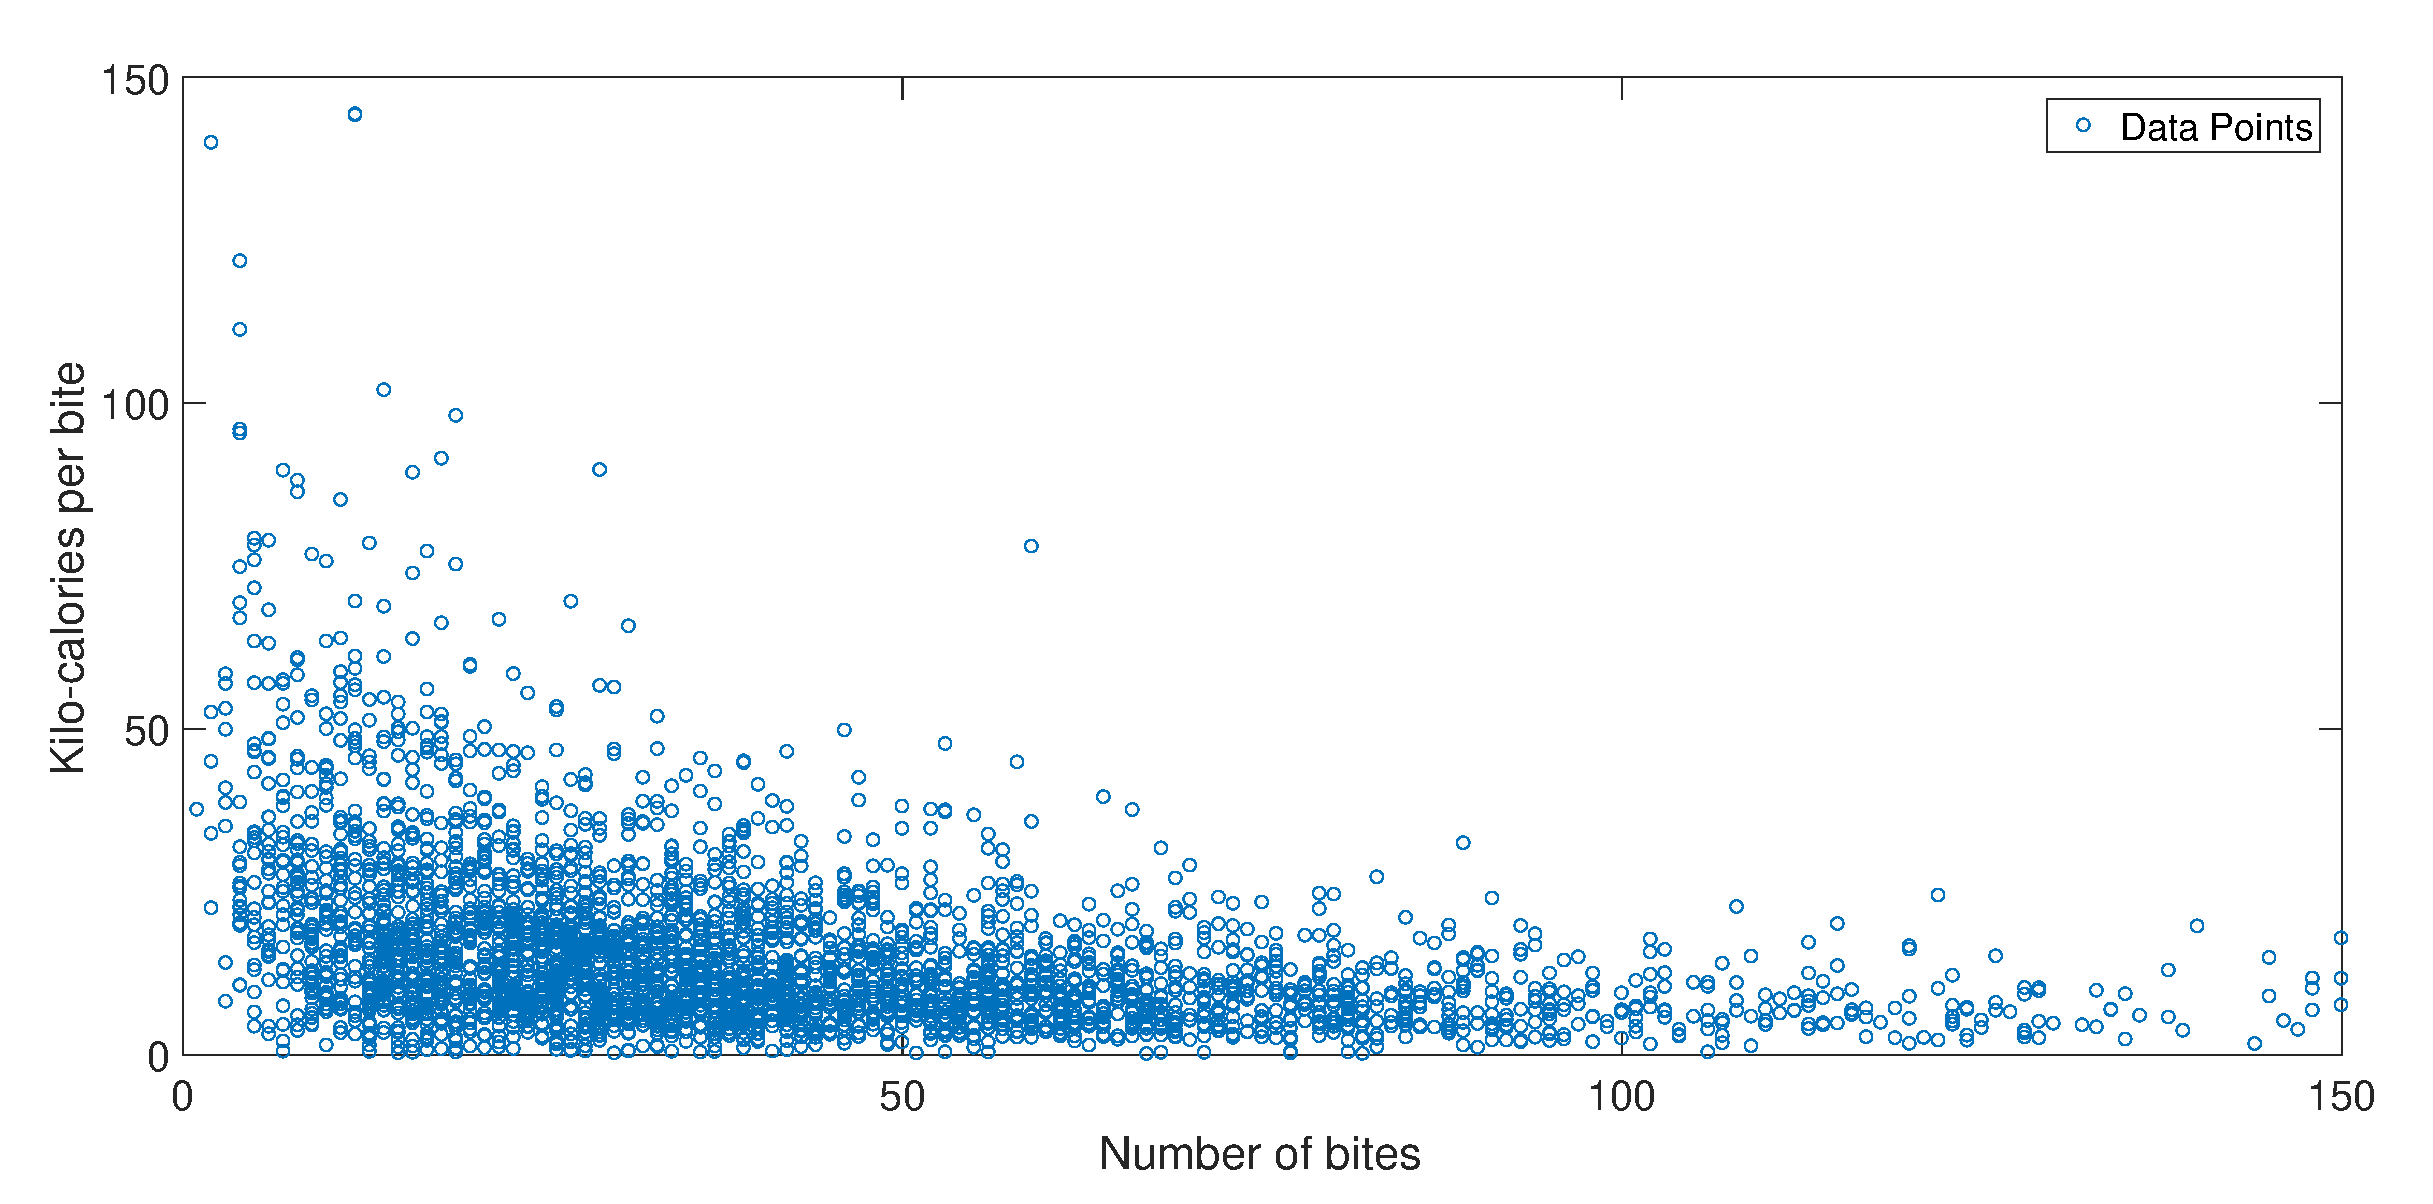
\includegraphics[width=\textwidth]{dataC}
	\caption{Unprocessed Part 3 Data set }
	\label{fig:unproc}
\end{figure}
\noindent
Figure \ref{fig:unproc} is the raw data plot of bites taken in any meal against the kilo-calories consumed per bite, without any kind of data pre-processing. On general observation, we can say that bites taken has sort of an exponential relationship with the calories consumed. That is, the calorie per bite is drops exponentially as the number of bites taken increases. It has to be kept in mind that the total number of calories consumed per meal is not effected by the number of bites taken and this is just a statistic of the calories consumed per bite for that meal. \\

\begin{figure}[t]
\centering
	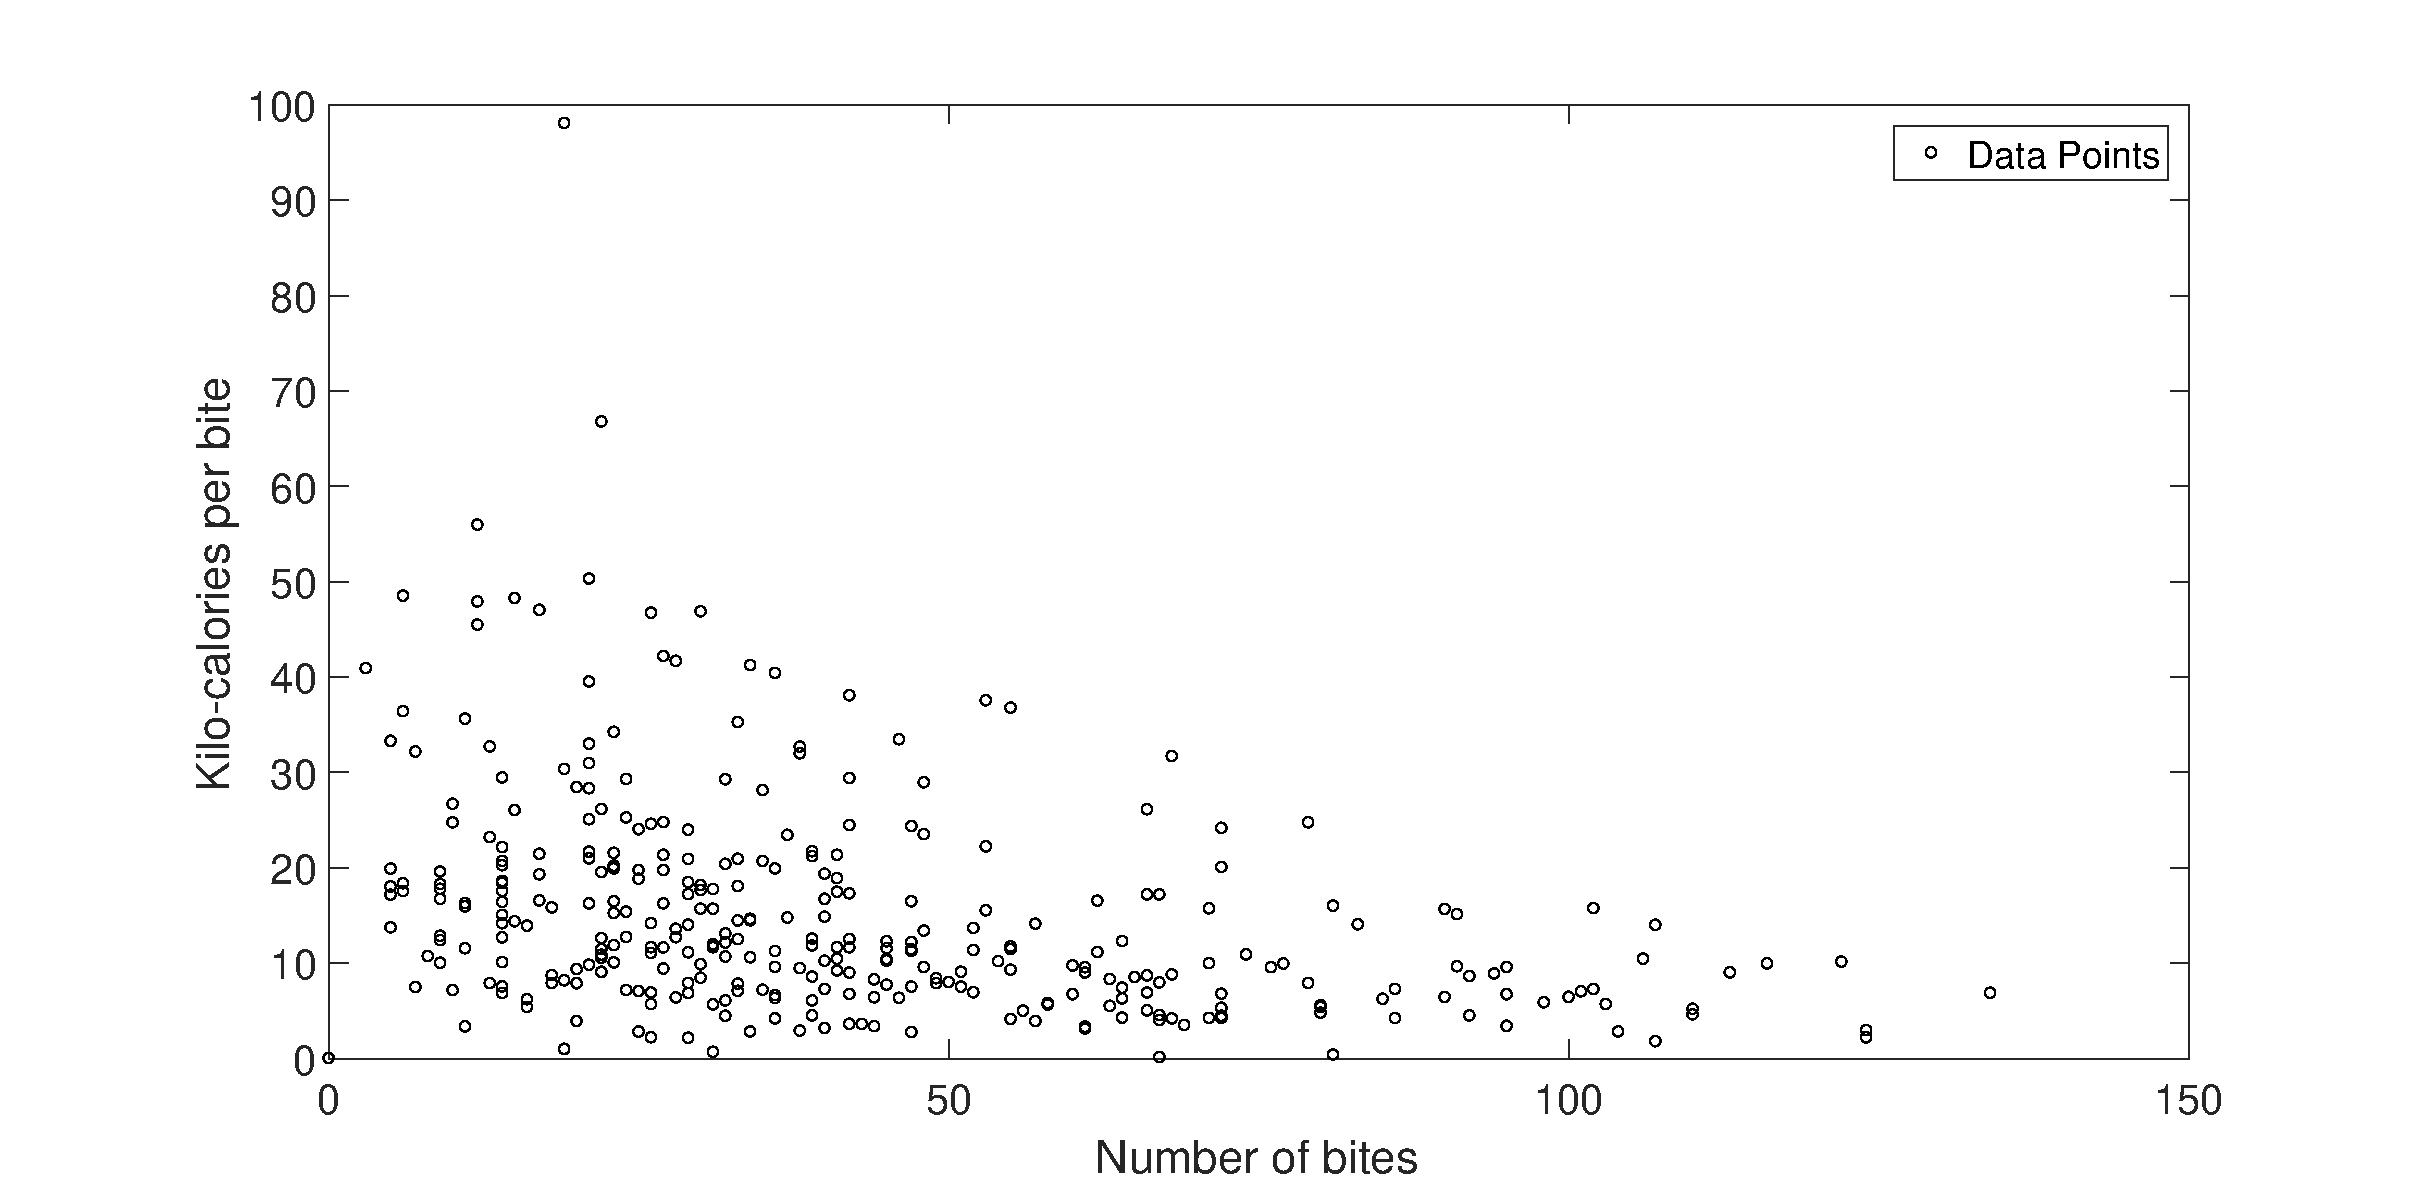
\includegraphics[width=\textwidth]{dataC_reduced}
	\caption{Plot of pre-processed Part 3 data }
	\label{fig:proc}
\end{figure}
\noindent
The raw data shown in Figure \ref{fig:unproc} has a lot of redundancy. Multiple data points overlap and the visualization of the data is not efficient. Thus for the purpose of better visualization, we will purge few of these redundant data points. Figure \ref{fig:proc} shows the same statistics as before, Kilo calories consumed per bite against the number of bites taken, but instead of plotting the entire data set  every tenth data entry is considered. This removes a lot of overlapping and the data interpretation becomes easier.  \\
\\
First we will try to fit a 2D line to this model and see whether it is a good fit. But as the observation revealed, the relationship in this case is more of an exponential than linear. So we will also consider a power fit model of the form $y = ax^b$ and see if it fits better than linear 2D line. \\
\\
Now using the same procedure as explained in section \ref{ss:general} the value of the line parameters for this case was found to be [-0.1771, 23.4417]. Thus the linear line fit will be of the form 
\begin{equation}
y = -1.771(x) + 23.4417
\label{ans:C}
\end{equation} \\
Now we will try to fit a power model of the form:
\begin{equation}
y = ax^b
\label{eq:power}
\end{equation}
Equation \ref{eq:power} has two unknowns, \lq{}a\rq{} and \lq{}b\rq{} and the equation is not linear in terms of its parameters. In order to convert the model to a linear form, we will take log on both sides
\begin{equation}
log(y) = log(ax^b)
\label{eq:log}
\end{equation} \\
we know that $log(m*n) = log(m) + log(n)$ and also $log(m^n) = n* log(m)$. Thus on using these two logarithmic properties, equation \ref{eq:log} simplifies to:
\begin{equation}
log(y) = log(a) + log(x^b) 
\end{equation}
\begin{equation}
log(y) = log(a) + blog(x) \label{eq:loglinear}
\end{equation}
Equation \ref{eq:loglinear} can be re-weitten as :
\begin{equation}
v = k + bu
\label{eq:simplifiedloglinear}
\end{equation}
where,
\begin{equation}
v = log(y) \quad
k = log(a) \quad
u = log(x)
\end{equation}
We will formulate the matrices as specified in equation \ref{eq:matA}, equation \ref{eq:matx} and  equation \ref{eq:matb} : 
\begin{equation}
A = 
	\begin{bmatrix}
	log(x_1) & 1 \\
	. & . \\
	. & . \\
	log(x_N) & 1 	
	\end{bmatrix}
\end{equation}
\begin{equation}
x = 
	\begin{bmatrix}
	a \\
	b 	
	\end{bmatrix}
\end{equation}
\begin{equation}
b = 
	\begin{bmatrix}
	log(y_1) \\
	. \\
	. \\
	log(y_N)
	\end{bmatrix}
\end{equation}

Now using equation \ref{eq:solution}, we get the values of the unknowns as a = 57.7128 and b = -0.4601. Thus the model will be of the form
\begin{equation}
y = (57.7128) x ^ {-0.4601}
\label{ans:Cpower}
\end{equation}

%%%%RESULTS************
\newpage
\section{Results}
In this section, we will go through the plots of the linear model fit and analyze them. \\
\begin{figure}[h]
\centering
	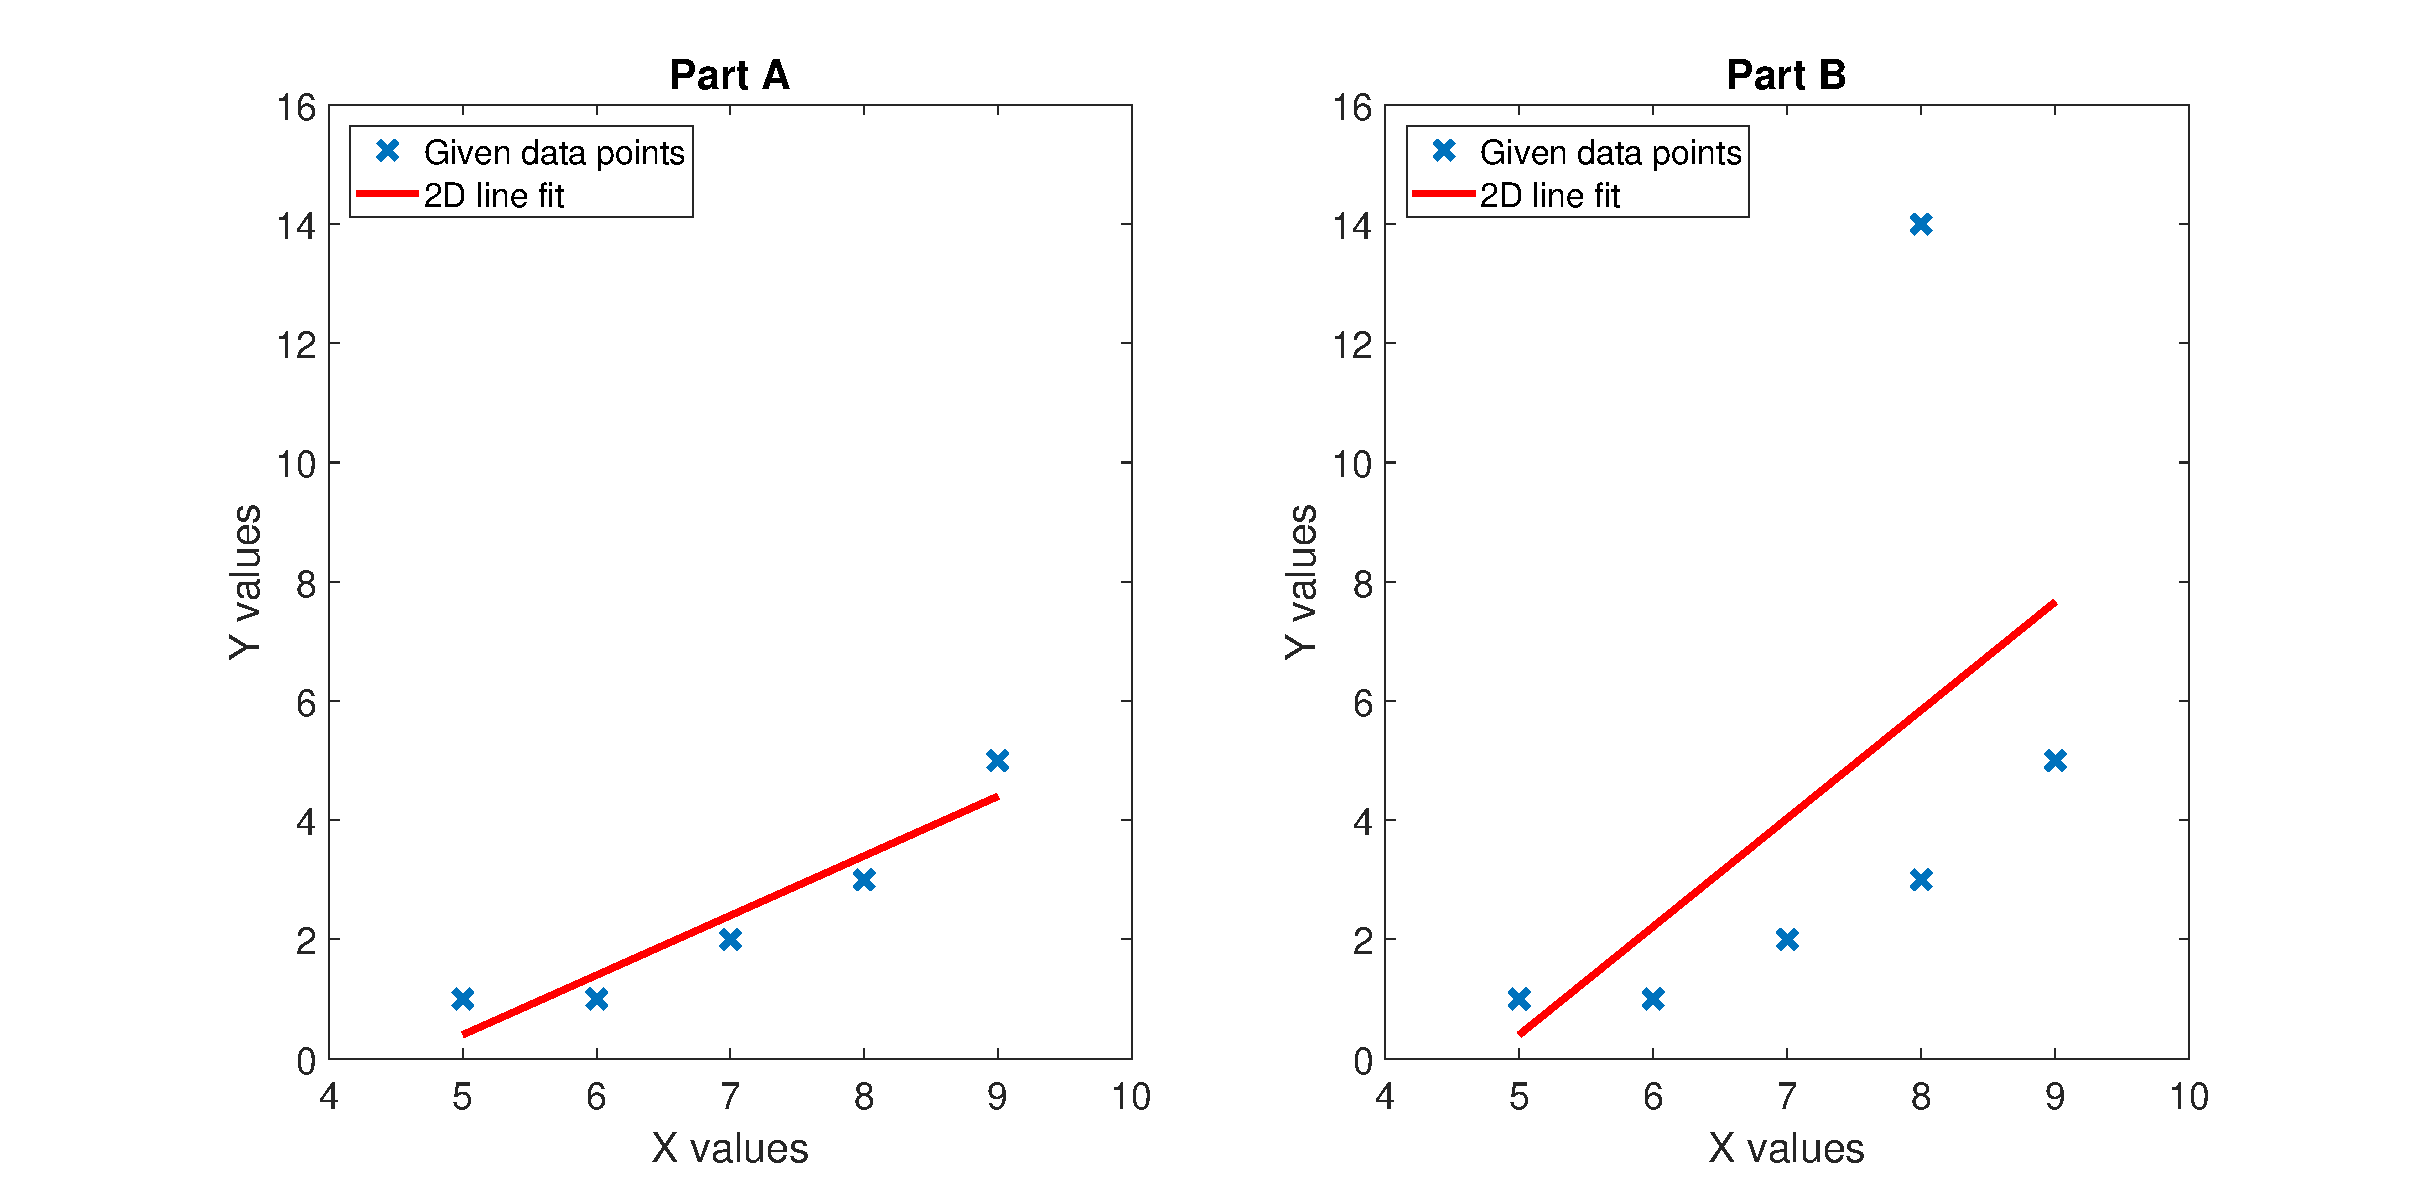
\includegraphics[scale=0.3]{resA}
	\caption{2D line fit for part A and Part B of lab}
	\label{res:1}
\end{figure}

\noindent
Figure \ref{res:1} shows the 2D line fit, whose parameters are given by equation \ref{ans:A} and equation \ref{ans:B}. Part A had 5 data points and the line fit model. Part B clearly shows the effect of the outlier point (8, 14) on the linear fitting model. The slope of the Part B model almost doubled due to the high y-value of the extra point. The slope for Part A was 1.00 which increased to 1.8154 when the extra data point was included.\\

\begin{figure}[h]
\centering
	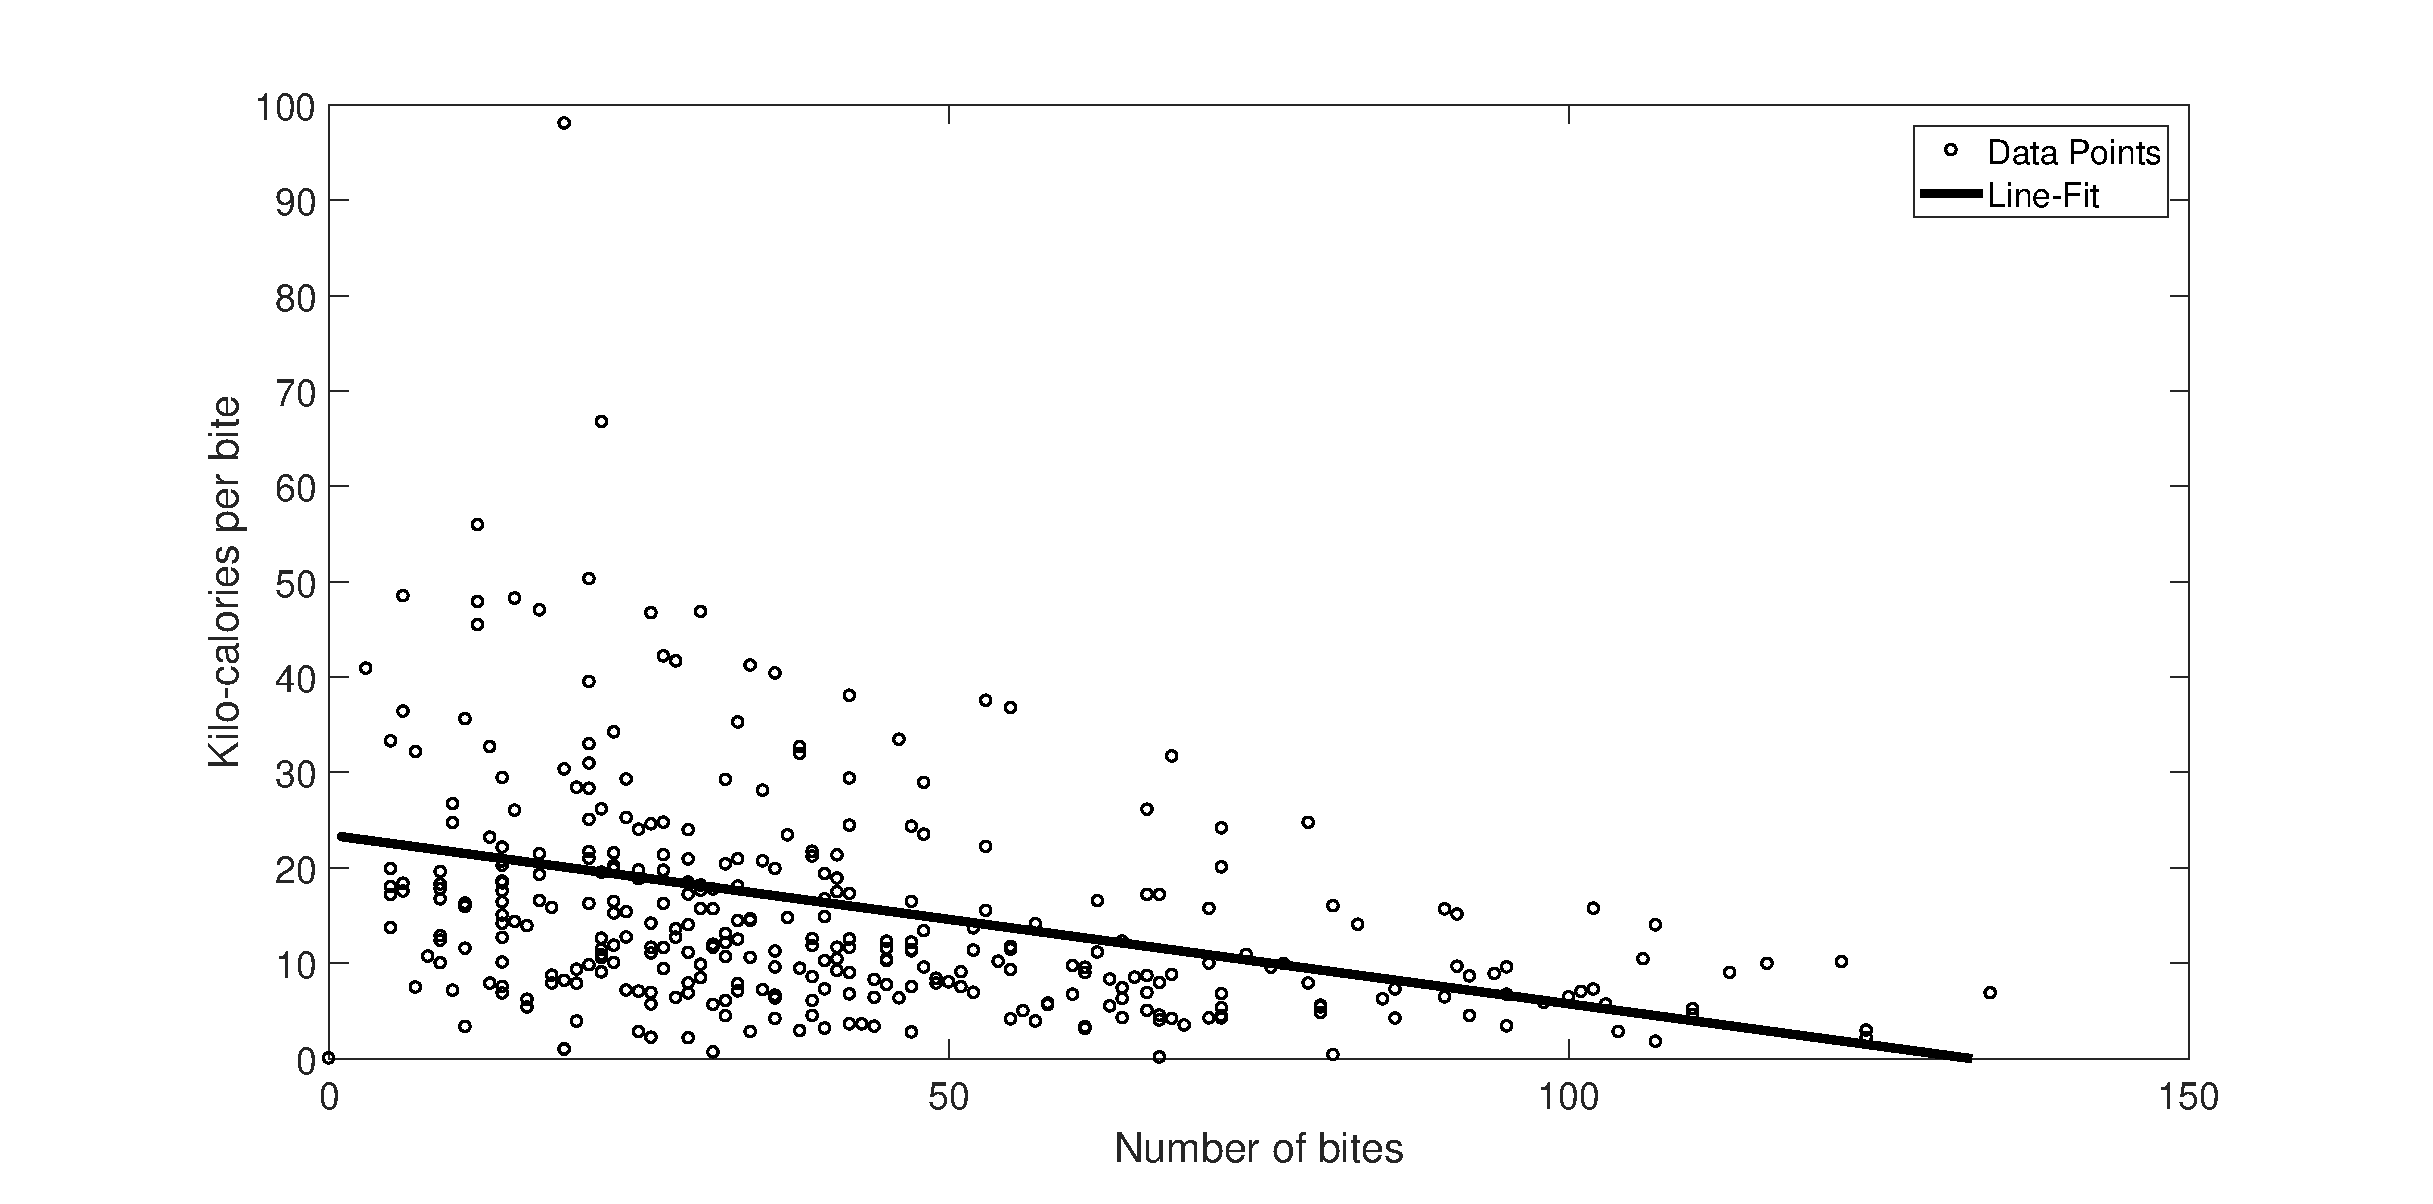
\includegraphics[scale=0.32]{resCline}
	\caption{2D line fit for part C of lab}
	\label{res:2}
\end{figure}
\noindent
Figure \ref{res:2} shows the line fit for the data set 2 used for part C of this lab assignment. The model is of the form $y = -0.1771(x) + 23.4417$ . This model is represented in the equation \ref{ans:C}  \\

\begin{figure}[h]
\centering
	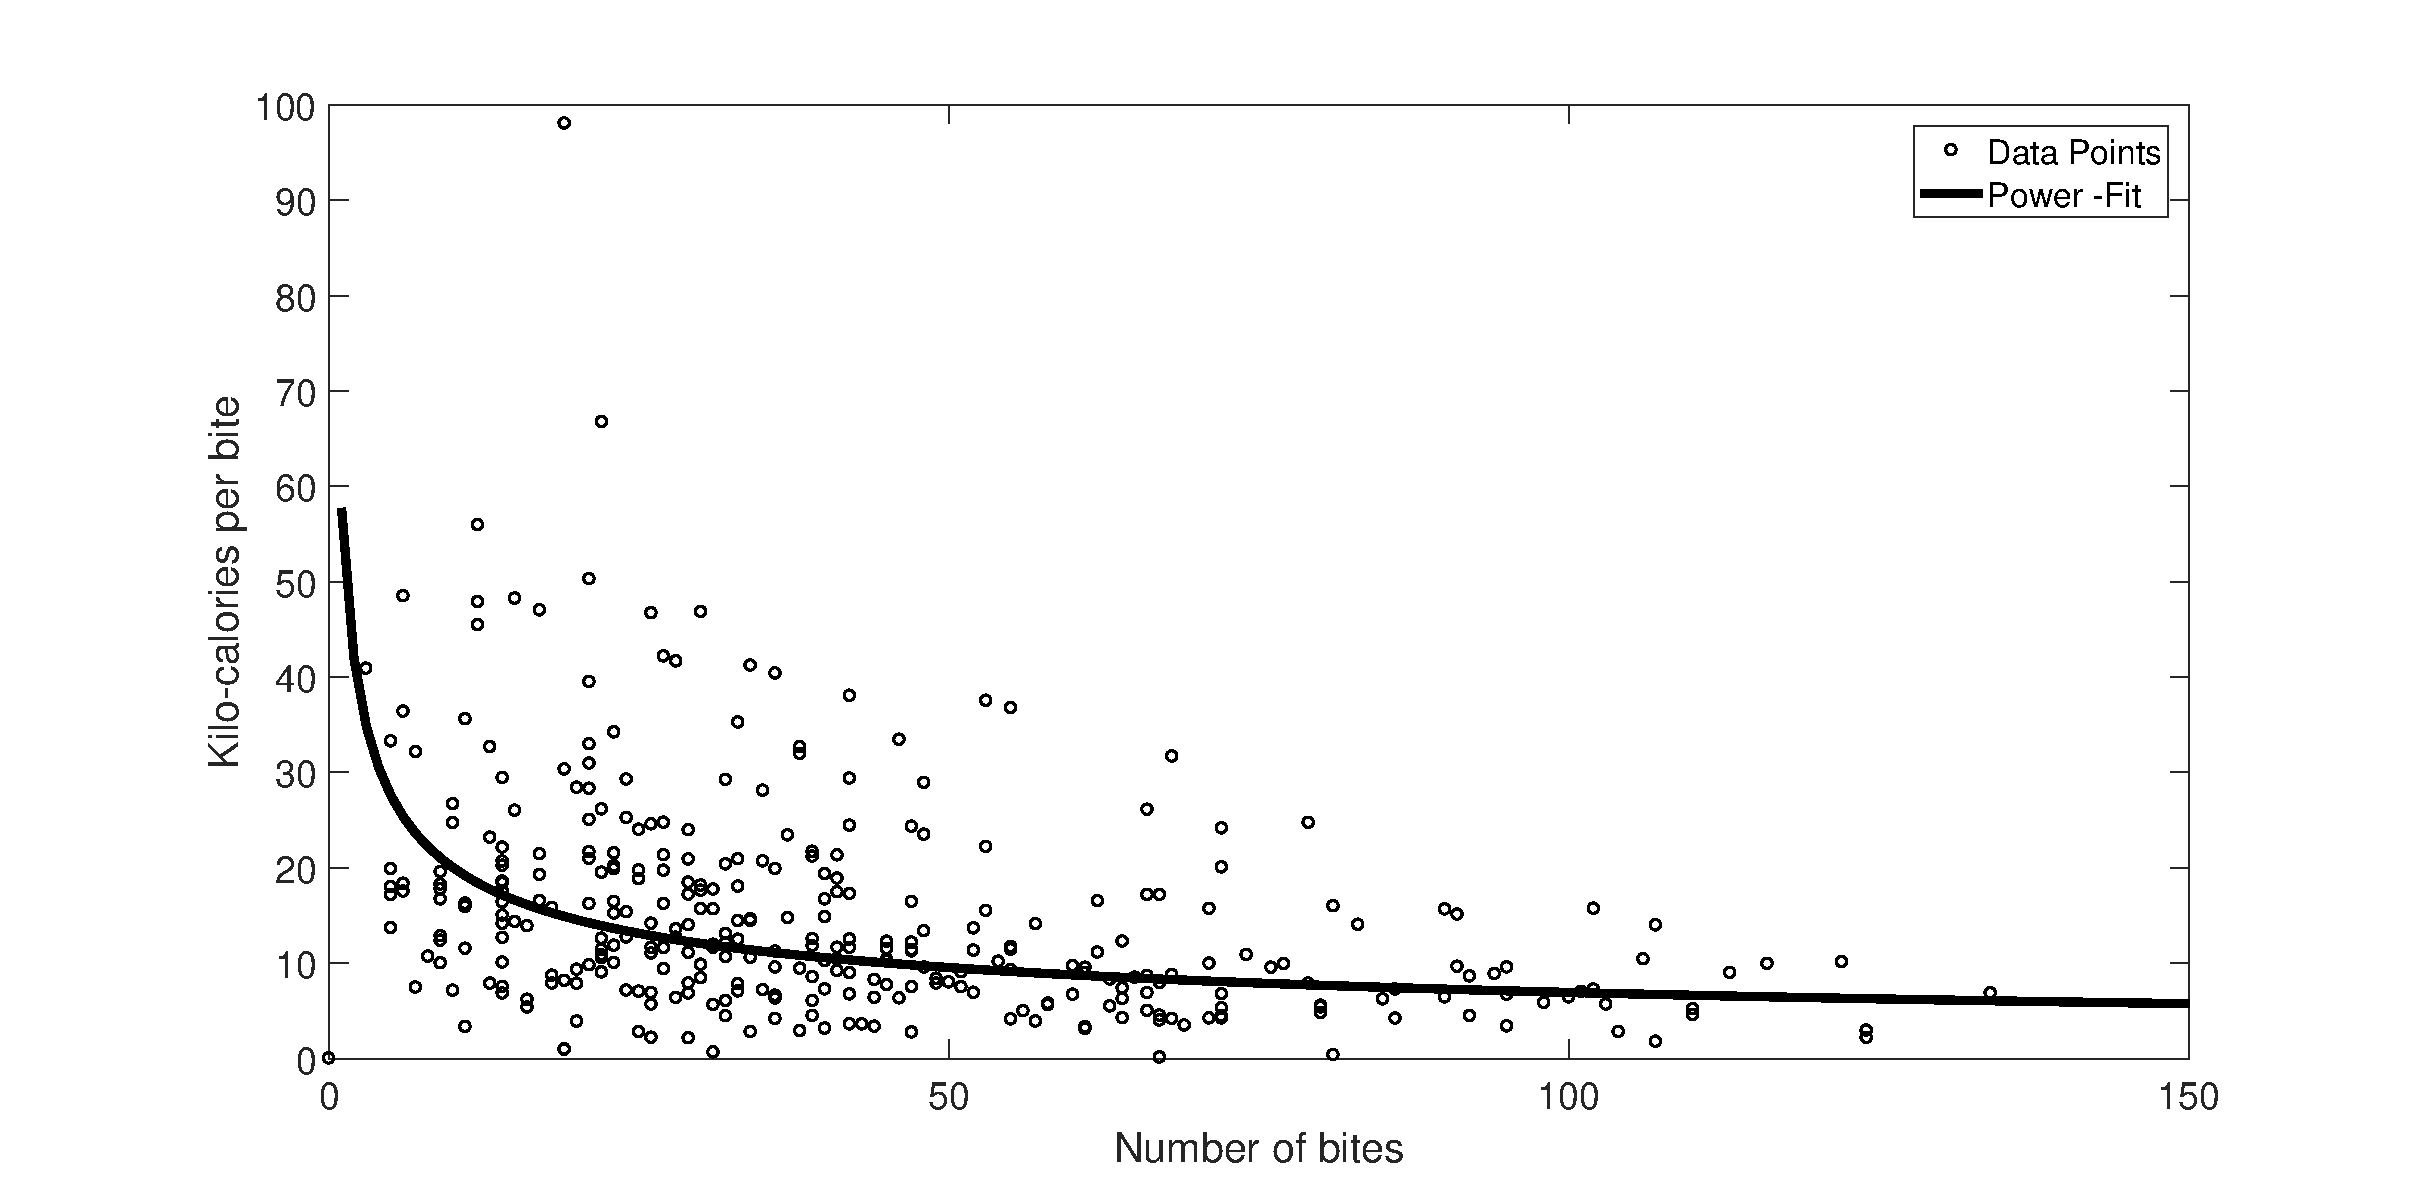
\includegraphics[scale=0.32]{resCpower}
	\caption{Power fit for part C of lab }
	\label{res:3}
\end{figure}
\noindent
Figure \ref{res:3} represents the power fit for the data set 2 used for part C of this lab assignment. The model shown in equation \ref{ans:Cpower}. This power model is defined as  $y = (57.7128)x^{(-0.4601)}$

\section{Conclusion}
In this lab, we derive the generalized solution, represented by equation \ref{eq:solution}, that can be used to fit any linear model that is of the form defined in equation \ref{eq:general} .
\subsection{Part A and Part B}
For this section of the lab assignment, we plotted the given data set A, which is shown in Figure \ref{fig:dataA} and Figure \ref{fig:dataB}. Our goal was to fit a 2D line and observe the effects of the extra point (8,14) on the line fit. \\
Figure \ref{res:1} shows the line fit. The graph in the left represents the part A fit and the right graph represents the part B. They have been arranged next to each other for the purpose of comparison. The line fir of part A gives a good approximation of the given data points. The addition of the outlier point, which has a high y-axis value, pulls the fitting line higher towards that point. The slope, which was 1.00 approximately doubles to 1.8154. This is the effect of the outlier point on the 2D line fit. 
\subsection{Part C}
Our goal for this section was to find a model for the data set represented by Figure \ref{fig:proc}. We choose to try out a linear 2D line fit shown in Figure \ref{res:2} and a power fit shown is Figure \ref{res:3}. The line fit was not a good approximation as the error around 0 - 50 bite range is high. The power model seems to be a much better fit compared to the 2D line. \\ Only two models were considered in this paper. It would be interesting to try out other models which could give better approximations than the ones discussed. 

\section*{References}
[1] \quad\url{http://statisticsbyjim.com/regression/difference-between-linear-nonlinear-regression-models/} \\

\noindent
[2] \quad\url{http://cecas.clemson.edu/~ahoover/ece854/lecture-notes/lecture-normeqs.pdf} \\

\noindent
[3] \quad\url{https://www.latex-tutorial.com/} \\

\noindent
[4] \quad\url{https://www.sharelatex.com/blog/latex-guides/beginners-tutorial.html} \\

%----------------------------------------------MATLAB LISTING TEMPLATE-------------------------

\lstset{language=Matlab,%
    %basicstyle=\color{red},
    breaklines=true,%
    morekeywords={matlab2tikz},
    keywordstyle=\color{blue},%
    morekeywords=[2]{1}, keywordstyle=[2]{\color{black}},
    identifierstyle=\color{black},%
    stringstyle=\color{mylilas},
    commentstyle=\color{mygreen},%
    showstringspaces=false,%without this there will be a symbol in the places where there is a space
    numbers=left,%
    numberstyle={\tiny \color{black}},% size of the numbers
    numbersep=9pt, % this defines how far the numbers are from the text
    emph=[1]{for,end,break},emphstyle=[1]\color{red}, %some words to emphasise
    %emph=[2]{word1,word2}, emphstyle=[2]{style},    
}


\section{Appendix}

\subsection{MATLAB Code}
\lstinputlisting{asg1.m}
%\lstinputlisting{find_a.m}
%--------------------------------------------------------------------------------------------------------

\end{document}
